\documentclass[]{elsarticle} %review=doublespace preprint=single 5p=2 column
%%% Begin My package additions %%%%%%%%%%%%%%%%%%%

\usepackage[hyphens]{url}

  \journal{Scientific Reports} % Sets Journal name

\usepackage{graphicx}
%%%%%%%%%%%%%%%% end my additions to header

\usepackage[T1]{fontenc}
\usepackage{lmodern}
\usepackage{amssymb,amsmath}
% TODO: Currently lineno needs to be loaded after amsmath because of conflict
% https://github.com/latex-lineno/lineno/issues/5
\usepackage{lineno} % add
\usepackage{ifxetex,ifluatex}
\usepackage{fixltx2e} % provides \textsubscript
% use upquote if available, for straight quotes in verbatim environments
\IfFileExists{upquote.sty}{\usepackage{upquote}}{}
\ifnum 0\ifxetex 1\fi\ifluatex 1\fi=0 % if pdftex
  \usepackage[utf8]{inputenc}
\else % if luatex or xelatex
  \usepackage{fontspec}
  \ifxetex
    \usepackage{xltxtra,xunicode}
  \fi
  \defaultfontfeatures{Mapping=tex-text,Scale=MatchLowercase}
  \newcommand{\euro}{€}
\fi
% use microtype if available
\IfFileExists{microtype.sty}{\usepackage{microtype}}{}
\usepackage[margin=3cm]{geometry}
\usepackage[]{natbib}
\bibliographystyle{plainnat}

\ifxetex
  \usepackage[setpagesize=false, % page size defined by xetex
              unicode=false, % unicode breaks when used with xetex
              xetex]{hyperref}
\else
  \usepackage[unicode=true]{hyperref}
\fi
\hypersetup{breaklinks=true,
            bookmarks=true,
            pdfauthor={},
            pdftitle={A rebuttal to Watters et al.~´2020 Long-term observations from Antarctica demonstrate that mismatched scales of fisheries management and predator-prey interaction lead to erroneous conclusions about precaution´},
            colorlinks=false,
            urlcolor=blue,
            linkcolor=magenta,
            pdfborder={0 0 0}}

\setcounter{secnumdepth}{0}
% Pandoc toggle for numbering sections (defaults to be off)
\setcounter{secnumdepth}{0}


% tightlist command for lists without linebreak
\providecommand{\tightlist}{%
  \setlength{\itemsep}{0pt}\setlength{\parskip}{0pt}}




\usepackage{booktabs}
\usepackage{longtable}
\usepackage{array}
\usepackage{multirow}
\usepackage{wrapfig}
\usepackage{float}
\floatplacement{figure}{H}
\newcommand{\pandocbounded}[1]{#1}
\usepackage{colortbl}
\usepackage{pdflscape}
\usepackage{tabu}
\usepackage{threeparttable}
\usepackage{threeparttablex}
\usepackage[normalem]{ulem}
\usepackage{makecell}
\usepackage{xcolor}
\usepackage{booktabs}
\newcommand{\blandscape}{\begin{landscape}}
\newcommand{\elandscape}{\end{landscape}}
\usepackage{float} \floatplacement{figure}{H}
\newcommand{\beginsupplement}{\setcounter{table}{0}  \renewcommand{\thetable}{S\arabic{table}}     -   - \setcounter{figure}{0} \renewcommand{\thefigure}{S\arabic{figure}}}
\usepackage{booktabs}
\usepackage{longtable}
\usepackage{array}
\usepackage{multirow}
\usepackage{wrapfig}
\usepackage{float}
\usepackage{colortbl}
\usepackage{pdflscape}
\usepackage{tabu}
\usepackage{threeparttable}
\usepackage{threeparttablex}
\usepackage[normalem]{ulem}
\usepackage{makecell}
\usepackage{xcolor}



\begin{document}


\begin{frontmatter}

  \title{A rebuttal to Watters et al.~´2020 Long-term observations from
Antarctica demonstrate that mismatched scales of fisheries management
and predator-prey interaction lead to erroneous conclusions about
precaution´}
    \author[1]{Andrew Lowther%
  %
  }
  
    \author[2]{Ulf Lindstrøm%
  %
  }
  
    \author[3]{Bjørn Krafft%
  %
  }
  
      \cortext[cor1]{Corresponding author}
  
  \begin{abstract}
  Characterising the impact of human activities on wildlife is a key
  function of applied science. In the Antarctic Peninsula, the fishery
  for Antarctic krill has been operating for over half a century, and
  concerns that fishery-driven localised depletion of krill around
  pygoscelid penguin colonies could have deleterious effect on their
  performance and demographic trends have been raised. One study
  utilises 30 years of penguin foraging and reproductive performance of
  penguins at two colonies in the South Shetland Islands matched against
  acoustic measurements of krill biomass and krill catches at the gSSMU
  scale \citep{Watters2020}. Herein we provide an assessment of the
  efficacy of this approach in drawing conclusions as representing sound
  scientific advice, given that the study in question is now being used
  as such. We demonstrate that several underlying assumptions in the
  Watters et al.~2020 study are contrary to the published scientific
  literature and not supported by the data provided by the authors
  themselves. When the modelling appraoch is reformulated to account for
  these inaccuracies, we demonstrate that the impact on penguin
  performance of fishing activity is greatly reduced, and that the
  dominant driver of penguin performance is the Oceanic Niño Index. We
  conclude that the original study should be treated with caution when
  used as a basis for fisheries management advice.
  \end{abstract}
  
 \end{frontmatter}

\section{Introduction}\label{introduction}

Concerns over the potential impact of localised depletion of krill
through concentrated fishing effort on krill-dependent predators has
been a topic of debate within the Antarctic science community for many
years. Recently, one study has been presented that suggest that local
harvesting rates can impact predator performance to the same degree as
poor environmental conditions (Watters, Hinke, and Reiss 2020) by
matching various performance indices of krill-dependent penguins
relative to estimates of krill biomass, fishing pressure and broad scale
climate variability. The penguin performance indices were collected at
two sites (Cape Shireff on Livingstone Island and Copacabana on King
George Island, South Shetland Islands; Figure 1) in the period 1982 -
2016 whereas krill abundance data, which cover the at-sea distributions
of chinstrap, gentoo and Adélie penguins, were collected during summer
(1996 - 2011) and winter (2012, 2014 and 2015). By drawing in monthly
krill catches from Catch and Effort data reported to CCAMLR and climate
data (ONI), the authors use a hierarchical analysis of variance approach
to estimate the variance in these indices as a function of Local Krill
Biomass (LKB), Local Harvesting Rates (LHR; the ratio of krill catch to
LKB) and the Oceanic Niño Index (ONI). The study drew the conclusion
that local harvesting levels of krill adversely impact penguins, and the
degree of impact can either be similar to that of poor environmental
conditions or have a synergistic impact when high local harvesting
coincides with poor conditions. The conclusions of this paper, which at
the time of writing has accumulated 162 citations, have been used by
CCAMLR in support of developing Marine Protected Area proposals and
fisheries management strategies as well as being used in the review
process of the Marine Stewardship Council fisheries certification
process for Antarctic krill. In other words, the outcomes of this study
have been propagated into geopolitical and socioeconomic environments
that are having real-world impacts beyond a scientific debate. However,
we have identified six critical issues that undermine the validity
of~Watters et al.~(2020). We provide a brief description of the
background behind each issue and a summarizing statement of the problem.

\subsection{\texorpdfstring{\emph{Continuing spatial and temporal
mismatches predators and fishing
activity}}{Continuing spatial and temporal mismatches predators and fishing activity}}\label{continuing-spatial-and-temporal-mismatches-predators-and-fishing-activity}

A key goal for Watters et al.~(2020) was to highlight the consequences
of mismatching scales at which the Antarctic krill fishery is managed
with the scales at which ecological interactions between fishing
extractions and dependent predators occur. To do this, the authors
created two strata aligned with groups of SSMU (gSSMU); gSSMU \#1
including those SSMU inside the Bransfield Strait (APBSE and APBSW) and
gSSMU \#2 incorporating SSMU north of the South Shetlands, including
Elephant Island (APDPE, APDPW and APEI) represented in Figure 1. These
gSSMU cover and , respectively, and are used to characterise both krill
biomass and harvesting rates that are ``local'' to the penguin colonies
for which performance data are used. The reasoning behind scaling to
gSSMU are linked to the foraging behaviour of the penguins for which
performance data area available i.e.~breeding, adult pygoscelids. The
authors cite Hinke et al.~(2017) as the evidence supporting usage of the
two gSSMU as appropriate strata. Pygoscelid penguins also exhibit
staggered breeding, with Adélies commencing first, followed by
chinstraps then gentoos (Black 2016). Adélie penguins are the first to
fledge their chicks and thus cease to be centrally foraging, typically
departing early February for their moulting grounds on the sea ice.
chinstrap penguins depart for a pre-moult foraging trip towards the
start of February and return to land in order to moult, before departing
again for their overwinter trip mid-March (Hinke et al.~2015); Hinke et
al.~2019). Conversely, gentoo penguins appear to remain near their
breeding colonies overwinter (Korczak-Abshire et al.~2021).

\emph{The model used by Watters et al.~(2020) presumes that penguins
occupy the entire gSSMU they are assigned to throughout the entire
year.}

\subsection{\texorpdfstring{\emph{Unsupported ecological
assumptions}}{Unsupported ecological assumptions}}\label{unsupported-ecological-assumptions}

The study's conclusions are also compromised by~unvalidated ecological
assumptions, particularly the assertion that~krill biomass at spatial
scales relevant to penguins varies with the phase of the Southern
Annular Mode (SAM). While SAM is known to influence large-scale
atmospheric circulation and sea ice extent (REF), its~direct
relationship to local krill biomass, especially at the scales relevant
to penguin foraging, has~not been empirically validated. The assumption
that SAM-driven variability in krill biomass uniformly affects penguin
performance across broad regions~ignores the complexity of local
oceanographic and biological processes. For instance,~krill recruitment
and aggregation~are influenced by a multitude of factors,
including~local prey availability, predation pressure, and fine-scale
hydrodynamic features, which are not captured by SAM alone (REF).
Without robust empirical support for this assumption, the study's
findings regarding the~interaction between climate, krill biomass, and
penguin performance remain~speculative. Addressing this gap
requires~finer-scale data~on krill distribution and environmental
drivers to validate, or refute, the proposed mechanisms underlying the
study's conclusions.

\emph{KEY PROBLEM STATEMENT - JAVIER}

\subsection{\texorpdfstring{\emph{Coding
errors}}{Coding errors}}\label{coding-errors}

A~coding error~further distorts the study's findings: the ``Worst Case''
scenario is described in the text as having a~neutral Oceanic Niño Index
(ONI)~but is incorrectly coded using a~warm ONI~parameter set
(Supplementary Material 1, lines 661--663). This misclassification
affects the interpretation of the model's outputs, particularly the
marginal probabilities associated with the ``Worst Case'' scenario.

\emph{Structural coding errors have created misleading results presented
in the published article.}

\subsection{\texorpdfstring{\emph{Omission of competing
species}}{Omission of competing species}}\label{omission-of-competing-species}

Another significant limitation of~Watters et al.~(2020)~is its~failure
to account for competing krill-dependent predators, such as~recovering
whale populations~(Baines et al.2021; Biuw et al.~2024) and~migratory
male Antarctic fur seals (Lowther et al.2020). These species~compete
directly with penguins for krill, particularly in key foraging areas
like the Bransfield Strait and Gerlache Strait (e.g.~Hückstädt et al.
2012; Johannessen et al.~2022). By ignoring the presence and consumption
demands of these predators, the study~overestimates the relative impact
of the krill fishery~on penguin performance. For example,~whales and
seals~can substantially reduce local krill availability, potentially
exacerbating any effects of fishing pressure. Without considering these
competing factors, the study's conclusions about the~impacts of
localized krill harvesting~on penguins are~incomplete and potentially
misleading. A comprehensive assessment of fishery impacts must
incorporate the~full suite of krill-dependent predators~to accurately
evaluate competition dynamics and their consequences for penguin
populations.

T\emph{he model used by Watters et al.~(2020) neglects the impact of
recovering populations of large-bodied krill eating predators that
overlap in time and space with penguins beyond a cursory discussion.}

\subsection{\texorpdfstring{\emph{Model
bias}}{Model bias}}\label{model-bias}

The analysis in~Watters et al.~(2020)~suffers from~two critical
methodological flaws~that undermine its conclusions. First, the model
includes~both Local Krill Biomass (LKB) and Local Harvest Rate (LHR)~as
separate predictors, despite LHR being mathematically derived from LKB
(LHR = Catch / LKB). This~structural
confounding~introduces~multicollinearity, making it impossible to
isolate the independent effects of krill availability and fishing
pressure on penguin performance. For example, areas with low LKB will
inherently yield higher LHR values even for modest catches, artificially
inflating the perceived impact of fishing pressure.

\emph{PROBLEM STATEMENT - ULF}

\subsection{\texorpdfstring{\emph{Over-reliance on broad-scale climate
indices}}{Over-reliance on broad-scale climate indices}}\label{over-reliance-on-broad-scale-climate-indices}

A further limitation of~Watters et al.~(2020)~is its~reliance on
macroscale climate indices, such as the~Oceanic Niño Index (ONI)~and
the~Southern Annular Mode (SAM), to explain variability in krill
availability and penguin performance. the utilisation of broad-scale
climatological phenomena to characterise impacts at scales that
predators are dependent upon is problematic. The Amundsen Sea Low (ASL)
is the dominant climate feature for the western Antarctic Peninsula. The
El Niño-Southern Oscillation (captured in the ONI predictor) modulates
the ASL, with El Niño (La Niña) shallowing (deepening) its pressure,
causing more northwesterly (southeasterly) winds and upwelling
(restricted influx) of Circumpolar Deep Water onto the shelf. The SAM
also influences the pressure of the ASL, with the current trend of
negative SAM constructively (destructively) interfering with ASL when in
phase with El Niño (La Niña) events (e.g.~Clem et al.~2016). The result
is a set of above-surface climate conditions that drive changes in water
mass intrusion that is in turn dependent on interactions between two
climate processes as well as the geographical orientation of the
coastline involved, all of which have been shown to impact the foraging
trajectories and trip durations of Chinstrap penguins (Andrew D. Lowther
et al.~2018). The bathymetry of the Antarctic Peninsula, which also
influences the hydrographic conditions, is complex particularly at
scales that are important to centrally-foraging predators such as
penguins. The structuring of krill aggregations in time and space in the
WAP have also been linked to mesoscale circulation processes (Santora et
al.~2012), which are unlikely to be uniformly affected by macroscale
processes given variation in local bathymetric and coastal orientation.
It is also worth noting that the study considers neither the impact of
climate on the terrestrial breeding grounds, such as chick mortality
through ``wetting down'' by increased rainfall (Chapman et al.~2011) nor
the unaccounted-for measurement inaccuracies in the foraging trip
durations used by Watters et al.~2020 (Lowther et al.~2015). While these
indices provide useful insights into large-scale atmospheric and
oceanographic patterns, they~fail to capture the finer-scale
processes~that directly influence krill distribution and predator-prey
interactions. For example,~mesoscale oceanographic features, such as
local upwelling, sea ice dynamics, and bathymetric influences, play a
critical role in determining krill aggregation and accessibility to
penguins (REF). However, these processes operate at spatial and temporal
scales that are~not adequately reflected~by broad indices like ONI or
SAM (REF). As a result, the study's conclusions about the impacts of
climate variability on penguin performance may be~oversimplified or
misrepresented, particularly in regions where local environmental
conditions deviate from large-scale climate patterns. This overreliance
on coarse climate indices~limits the study's ability to accurately
assess~the true drivers of krill availability and, consequently, penguin
responses to environmental change. As such, the general structure of the
study does not appear to be appropriate for answering the research
questions raised.

\emph{The model used by Watters et al.~(2020) relies exclusively on
ocean-scale climate indices as environmental predictors of LKB and
penguin performance.}

\subsection{}\label{section}

Herein, we conduct analyses and discuss these to demonstrate the
inappropriate or unsupported conclusions related to Issues \#1 to \#3
and the potential impact that Issue \#4 raises in understanding the
drivers of penguin performance. We then discuss Issues \#5 and \#6
qualitatively, with no associated numerical analyses.

\section{Materials and Methods}\label{materials-and-methods}

\subsection{\texorpdfstring{\emph{Continuing spatial and temporal
mismatches}}{Continuing spatial and temporal mismatches}}\label{continuing-spatial-and-temporal-mismatches}

predators and fishing activity We use the Argos-CLS PTT telemetry data
provided by the supporting studies in Watters et al.~(2020) to
characterise the actual at-sea habitat used, in the context of the
relative stage of breeding for each species, though we also recommend
Warwick-Evans et al.~(2018) and Lowther et al.~(2018) amongst other
work, for further quantification of foraging behaviour of breeding
penguins in this area. For each species, we refrain from undertaking
extensive state-space modelling of location errors and merely exclude
locations with a ``Z'' error class, accepting the remaining locations
had varying degrees of uncertainty around them. We then calculated the
99\% Minimum Convex Polygon (home range) using the R package
adehabitatHR and calculate their associated areas in , with the
resulting MCP likely being larger than the area actually exploited,
given the remaining inaccuracy in the underlying locations used.

We then scale the gSSMU LKB to the SSMU that the summer tracking data
indicate penguins occupied. To do this, we calculate the area () of the
SSMU for which the predator occupies and the gSSMU to which it is
assigned, then create a scaling ratio. For example, we scale LKB for
Cape Shireff chinstrap penguins solely to ADPDW (Figure 1) by
multiplying the gSSMU LKB by the areal ratio of ADPDW/gSSMU \#2. We then
select the corresponding SSMU catch values provided in Watters et al.
(2020) (Supplementary Info) to estimate SSMU-scale LHR. We also caution
that while considering the gSSMU scale of harvesting as inappropriate
for ``local'' effects, even the SSMU-scale catch levels likely do not
reflect pressures at scales relevant to breeding penguins. The authors
place LKB/LHR values in March into the ``summer'' period, thus
effectively incorporating fishing pressure into the summer breeding
season in the context of penguin performance metrics. However fishing
effort over the period that performance indices are available is not
uniform over the thirty year period, with catch over the preceding
decade tending towards a nonlinear increase from the middle of March and
three years where catch rates increased rapidly from the beginning of
March (Figure 4). Given the highly variable rates of catch throughout
the study period, we run scenarios that classify March as either summer
or winter to reflect the linkage between March and the breeding state of
penguins i.e.~Adélie and chinstrap penguins have either migrated out of
the area or have ceased to be centrally foraging species by March (HINKE
REFS GALORE, INCLUDING 2025 Scientific Reports).

Thus we reformulate the underlying assumptions above into a new model
construct, in which performance indices from gentoo, chinstrap and
Adélie penguins during the summer are included, but Adélie and chinstrap
penguins cease to be centrally foraging species after breeding and
migrate out of the area. The performance indices are matched in space
and time but using SSMU level estimates of LKB and LHR. We re-run the
model twice 1) using gappy survey data and 2) including imputed values
for LKB in years where survey data are missing. We further consider two
alternatives for considering March, either in a) summer or b) winter on
each model run.

We present the outputs both in the same boxplot format as Figure 2 in
the original manuscript, and as individual cases grouped and
colour-coded as ONI ``warm'' ( 0.5; red), ONI ``neutral'' (-0.5
\textless{} ONI \textgreater{} +0.5; white) and ONI ``cold''
(\textless{} -0.5; blue). We also recreate the original marginal
probabilities in Table 1 of Watters et al.~(2020), and two additional
tables in the same format with the probabilities extracted from our
reformulated model, the difference between the latter two tables
reflecting whether March is in summer or winter.

\subsection{\texorpdfstring{\emph{Unvalidated Ecological
Assumptions}}{Unvalidated Ecological Assumptions}}\label{unvalidated-ecological-assumptions}

\subsection{\texorpdfstring{\emph{Model coding
error}}{Model coding error}}\label{model-coding-error}

We also note an additional coding error that may influence how the
original, unmodified results are interpreted. In summarising the model
outputs into boxplots, the text in the paper seemingly classifies the
``Worst Case'' with ``neutral'' ONI ( oC \textless{} ONI \textless{} 0.5
oC; LKB \textgreater{} 1 Mt; and LHR 0.1) and the code relating to
developing the original manuscript Figure 2 uses Parameter set 36 from
the output dataframe, which actually reflects a ``warm'' ONI component
(\textgreater{} 0.5 oC; LKB \textgreater{} 1 Mt; and LHR 0.1). Yet the
discussion in Watters, Hinke, and Reiss (2020) also suggests that the
likelihood of their ``Worst Case'' includes future warming (see Figure 3
below)

We agree that any ``Worst Case'' should reflect ENSO conditions into the
future under a warming climate. However, climate change is likely to
increase ENSO in amplitude - both El Niño (ONI ``warm'') and La Niña
(ONI ``cold'') (Capotondi et al.~2015). How this increasing amplitude
can be integrated appropriately into the presented modelling framework
to match with long-term predicted mean performance of predators has not
been explored yet. As such, and for the sake of comparison with the
original study, we maintain the authors designation of ONI ``neutral''
when rendering the ``Worst Case'' boxplots, though caution that this is
unlikely to be a realistic assumption

\subsection{\texorpdfstring{\emph{Omission of competing
species}}{Omission of competing species}}\label{omission-of-competing-species-1}

In order to provide numerical context on the potential role baleen
whales and Antarctic fur seals may play in regulating penguin
performance, we conduct two analyses. Firstly, we use published
estimates of the time-evolving abundance and distribution of humpback
whales (Megaptera novaeangliae) throughout the Bransfield Strait
(Johannessen et al.~2022) to estimate the number of whales present in
the SSMU occupied by penguins from Copacabana. We then use conservative
per-capita consumption estimates (REF) to derive monthly krill
consumption rates and compare these to the SSMU krill catch provided in
Watters et al.~(2020). Secondly, we use per-capita krill consumption
rates for adult male Antarctic fur seals which are known to migrate into
the region from as early as January until the beginning of the following
summer breeding season (Lowther et al.~2020). The catch limit in the
management unit in which the Watters et al.~(2020) is conducted was
155,000tonnes/year, and we back-calculate the number of Antarctic fur
seals that would need to be present to at least equal the krill removal
rate of the fishery.

All analyses are conducted in the R statistical software environment (R
4.5.1), using the original data provided in Watters et al.~(2020) or in
the published articles cited as supporting evidence. To faciliate
reproducibility, the Supplementary Material from the original Watters et
al.~(2020) article and the Supplementary Material from all necessary
supporting articles are hosted in Zenodo repositories (record ID 5040114
and record ID 17347172). A dedicated R script allowing for these data
and scripts to be downloaded directly from the repositories is provided
in Appendix I. Fully annotated R code, highlighting the modifications
and justifications, as well as the code needed to fully reproduce the
figures and tables presented here, are also included in the Zenodo
repositories.

\section{Results}\label{results}

\subsection{\texorpdfstring{\emph{Continuing spatial and temporal
mismatches}}{Continuing spatial and temporal mismatches}}\label{continuing-spatial-and-temporal-mismatches-1}

Comparing the original model outputs with ours, relative to the ``Best
Case'', the probability of negative impacts to penguins due to high LHR
dropped precipitously from 93\% to 37\% (Table 3). In other words, when
considering the migration of penguins in accordance with their known
ecology (Figure 2), the relative probability of negative impact of LHR
drops from a near-certainty to 1-in-3 (Table 2 and 3). At this point, we
clarify that the probability of negative impact is not a measure of the
scale of the expected impact (i.e.~a measure of population decline), but
a measure of whether any negative impact is likely to occur. Given the
temporal separation between fishing and penguin breeding over the
preceding decade, our results are unsurprising.

\subsection{\texorpdfstring{\emph{Unvalidated Ecological
Assumptions}}{Unvalidated Ecological Assumptions}}\label{unvalidated-ecological-assumptions-1}

\subsection{\texorpdfstring{\emph{Model coding
error}}{Model coding error}}\label{model-coding-error-1}

\subsection{\texorpdfstring{\emph{Omission of competing
species}}{Omission of competing species}}\label{omission-of-competing-species-2}

\begin{verbatim}
• Figure 1: Impact of Spatial and Temporal Adjustments on Expected Penguin Performance. Illustrate the combined effect of spatial and temporal corrections on model outputs. Highlight that LHR impacts are overestimated in the original model.
\end{verbatim}

Content: • Boxplots~comparing expected penguin performance under: ◦
Original model~(gSSMU scales, Adélie/chinstrap penguins included in
winter, March as summer). ◦ Revised model~(SSMU scales, Adélie/chinstrap
penguins excluded in winter, March as winter). • Color-coded by ONI
conditions: ◦ Warm (≥0.5°C; red). ◦ Neutral (-0.5°C \textless{} ONI
\textless{} 0.5°C; white). ◦ Cold (\textless-0.5°C; blue).

\begin{verbatim}
• Table 1: Marginal Probabilities of Negative Impacts on Penguin Performance
\end{verbatim}

Content: • Comparison of marginal probabilities~for: ◦ Original
model~(Watters et al., 2020). ◦ Revised model~(spatial rescaling to
SSMU, temporal adjustments, March as winter). • What to include: •
Probability of negative impact from~high LHR~(original: 93\%; revised:
37\%). • Probability under~``Worst Case''~(neutral ONI, high LHR, high
LKB). • Dominance of~ONI effects~in revised model.

Unvalidated Ecological Assumptions • Figure 1: Relationship Between SAM
Phases and Local Krill Biomass (LKB). Visually confirm the~lack of
correlation~between SAM and LKB. Support the argument that~local
processes~(e.g., upwelling, bathymetry) are more influential than
broad-scale climate indices. Content: • Scatter plots or regression
plots~showing: ◦ SAM index values~(x-axis) vs.~Local Krill Biomass
(LKB)~(y-axis). ◦ Data points~for different SAM phases (positive,
neutral, negative). ◦ Regression line~with~R² and p-values~indicating no
significant relationship (F \textless{} 0.975, p \textgreater{} 0.33). •
Highlight:~Visual demonstration that~LKB does not vary predictably with
SAM phases.

\begin{verbatim}
• Table 1: Statistical Tests for SAM-LKB and Low LKB-Small Krill Relationships
\end{verbatim}

Content:

\section{Discussion}\label{discussion}

Our reanalysis of~Watters et al.~(2020)~reveals that the study's
conclusions are based on~assumptions not supported by empirical data. By
addressing~spatial and temporal mismatches,~unvalidated ecological
assumptions, and~methodological biases, we demonstrate that
the~perceived impacts of krill fishing on penguin performance are
significantly overestimated. Specifically, rescaling spatial units
from~gSSMUs to SSMUs~and accounting for~penguin migration
patterns~reduced the probability of negative impacts from high Local
Harvest Rates (LHR)~from 93\% to 37\%. Additionally, our findings
highlight that~broad-scale climate indices (ONI, SAM)~are less
influential than~local oceanographic processes~in determining krill
availability and penguin performance.

\subsection{\texorpdfstring{\emph{Spatial and temporal mismatches
undermine study
conclusions}}{Spatial and temporal mismatches undermine study conclusions}}\label{spatial-and-temporal-mismatches-undermine-study-conclusions}

The~spatial scales~used in Watters et al.~(2020) are~4--15 times
larger~than the actual foraging ranges of penguins. For example, Adélie
penguins forage within~1,139 nm², yet the study used~gSSMUs of
15,500--20,600 nm²~to define ``local'' krill biomass and harvest rates.
This mismatch leads to~overestimated localized depletion effects, as the
broad spatial units fail to capture the fine-scale interactions between
penguins and their prey. Similarly, the study's~temporal
assumptions~incorrectly associate winter fishing pressure with penguin
performance, despite Adélie and chinstrap penguins~migrating away from
breeding colonies by late February. By excluding these species from
winter analyses, we show that the~original model's conclusions about
seasonal fishing impacts are misassigned.

\subsection{\texorpdfstring{\emph{Unvalidated ecological
assumptions}}{Unvalidated ecological assumptions}}\label{unvalidated-ecological-assumptions-2}

Watters et al.~(2020) assumes that~krill biomass varies with the
Southern Annular Mode (SAM), yet our statistical tests reveal~no
significant correlation~between SAM phases and Local Krill Biomass
(LKB). Similarly, the assumption that~low LKB (\textless1 Mt) correlates
with small krill~is unsupported. The study's reliance on~SAM and
ONI~thus oversimplifies the complex, fine-scale interactions driving
krill-penguin dynamics. Additionally, the study overlooks the role of
krill life-stage dynamics~in shaping availability and accessibility for
penguins and other predators. Krill populations consist of~multiple size
classes and age cohorts, each with distinct spatial distributions,
seasonal behaviors, and energetic values for predators (REF). For
instance, small juvenile krill, which may dominate recruitment pulses,
are often~less energetically valuable~to penguins than larger, older
krill (REF). Seasonal and spatial variability in krill size structure
(e.g., due to recruitment events or environmental conditions) can
significantly influence predator performance (REF), yet these dynamics
are~not explicitly considered~in Watters et al.~(2020). By treating
krill biomass as a~homogeneous metric, the authors ignore critical
variations in krill quality and availability that may drive penguin
foraging success or failure. Addressing this gap
requires~life-stage-specific data~on krill distribution and predator
preferences to refine assessments of how fishing and environmental
changes affect penguin populations. Together, these oversights highlight
the need for~finer-scale ecological data~to validate, or refute, the
mechanisms underlying the study's conclusions.

\subsection{\texorpdfstring{\emph{Model coding
error}}{Model coding error}}\label{model-coding-error-2}

The~coding error~distorts the study's findings. The ``Worst Case''
scenario is described in the text as having a neutral Oceanic Niño Index
(ONI) but was incorrectly coded using parameters for a warm ONI. This
misclassification inflates the perceived severity of neutral ONI
conditions, leading to misinterpretation of the model's outputs,
particularly the marginal probabilities associated with the ``Worst
Case'' scenario. The coding error reduces the probability of negative
impacts from high LHR from 93\% to 37\% (Table 3). This adjustment
highlights that fishing pressure effects depend on krill abundance,
where low LKB amplifies the perceived impact of LHR, while high LKB
masks it. Furthermore, the revised model clarifies that the dominance of
ONI over LHR in driving penguin performance becomes evident when
structural biases are removed.

\subsection{\texorpdfstring{\emph{Omission of competing krill
predators}}{Omission of competing krill predators}}\label{omission-of-competing-krill-predators}

A major limitation of Watters et al.~(2020) is its~failure to account
for competing krill-dependent predators, such as~recovering whale
populations~and~migratory male Antarctic fur seals. Using available
abundance, distribution and consumption estimates for competing species,
we show that humpback whales consume over five times the amount of krill
than taken by the fishery per month. We show that the number of male
Antarctic fur seals required to match the LHR of the fishery for each
year of the study ranges from as few as zero to as many as 72,000 seals;
given the number of seals that are recorded at only two sites in the
South Orkney Islands (32,000 individuals) and their movements into the
Antarctic Peninsula are well documented (Lowther et al.~2020), there are
likely to be significant competitive interactions between migrating
seals and breeding penguins. The consumption by whales also overlaps
temporally with penguin breeding, unlike the fishery which since 2010
has shifted to a winter fishery (REF). Intuitively then, ignoring the
vast amount more krill removed by whales at the same time as breeding
penguins are foraging is likely to be greatly overestimating the
relative impact of fisheries removal on penguin performance. Future
assessments must incorporate~multi-species interactions~to accurately
evaluate the cumulative pressures on krill-dependent predators.

\subsection{\texorpdfstring{\emph{Model
Bias}}{Model Bias}}\label{model-bias-1}

The presence of~structural model bias~arising from the confounding
relationship between covariates (LHR and LKB; LHR=Catch/LKB) was not
explicitly explored in this study. This dependency, however, masks the
isolated effects of krill availability (LKB) and fishing pressure
(Catch) on penguin performance, potentially leading to misleading
conclusions about the relative importance of these factors. This
structural confounding in the model results in~artificial inflation of
fishing impacts~in areas with low LKB, where even modest catches yield
high LHR values, thereby exaggerating the perceived impact of fishing
pressure on penguin performance. Conversely, in areas with high LKB,
substantial catches may be masked because the same absolute catch
results in a lower LHR, underestimating the true effects of fishing.
This structural bias undermines the study's ability to disentangle the
true ecological drivers of penguin performance, necessitating a
reevaluation of the model's specifications and assumptions. These
findings underscore the necessity for methodological rigor in ecological
modeling. Future studies should avoid multicollinearity by using Catch
and LKB as separate predictors instead of LHR to isolate the effects of
fishing pressure and krill availability. Additionally, validating coding
and assumptions is crucial to ensure that scenario classifications align
with described conditions and prevent misinterpretation. Finally,
reevaluating model specifications to account for structural biases will
enable more accurate assessments of the impacts of fishing on predator
performance. 6 Over-reliance on broad-scale climate indices Watters et
al.~(2020) relies on~macroscale climate indices (ONI, SAM)~to explain
variability in krill availability, yet these indices fail to
capture~finer-scale oceanographic processes~(e.g., local upwelling, sea
ice dynamics) that directly influence krill aggregation. Our reanalysis
shows that~local environmental predictors~(e.g., sea ice concentration,
chlorophyll-a) explain more variance in penguin performance than ONI or
SAM. This over-reliance on broad-scale indices~limits the study's
ability to accurately assess~the true drivers of krill availability and
penguin responses to environmental change.

\subsection{\texorpdfstring{\emph{Implications for fisheries
management}}{Implications for fisheries management}}\label{implications-for-fisheries-management}

The~real-world implications~of Watters et al.~(2020) are substantial, as
its conclusions have influenced~CCAMLR's Marine Protected Area
proposals~and~fisheries certification processes. However, our findings
suggest that the study's~methodological limitations---spatial/temporal
mismatches, unvalidated assumptions, and omitted
competitors---compromise its validity as a management tool. We recommend
that future assessments: 1. Use~spatial scales aligned with penguin
foraging ranges~(SSMUs rather than gSSMUs). 2. Account for~penguin
migration and seasonal fishing effort. 3. Incorporate~competing
predators~and~local environmental drivers. By addressing these issues,
managers can develop~more robust, evidence-based strategies~for
balancing krill fisheries with predator conservation.

\subsection{\texorpdfstring{\emph{Broader concerns and future
directions}}{Broader concerns and future directions}}\label{broader-concerns-and-future-directions}

While Watters et al.~(2020) raises important questions about fishery
impacts, its~boundary conditions, focusing solely on fishing and
climate, are~inadequate~for disentangling the~relative impacts of
multiple stressors~on krill-dependent predators. Over~20 years ago,
CCAMLR acknowledged that its~CEMP program~could not distinguish between
fishing and climate effects (REF), yet no modifications have been made.
Moving forward,~integrated monitoring programs~that account
for~competition, local oceanography, and fine-scale predator-prey
interactions~are essential for informing~sustainable fisheries
management~in the Antarctic.

\subsection{\texorpdfstring{\emph{Conclusion}}{Conclusion}}\label{conclusion}

Our reanalysis demonstrates that the~conclusions of Watters et al.
(2020) are overly pessimistic~due to~spatial/temporal mismatches,
unsupported ecological assumptions, omitted confounding impacts of
competitive predators and methodological biases. While~climate
variability (ONI)~remains a dominant driver of penguin performance,
the~impacts of krill fishing are far less severe~when analyzed
at~ecologically relevant scales. To ensure~objective scientific
advice~for CCAMLR, future studies must adopt~finer spatial/temporal
resolutions, incorporate~competing predators, and avoid~structural
biases. Only then can we accurately assess the~true impacts of
fishing~on Antarctic krill-dependent predators.\newpage

\begin{table}[ht]
\centering
\resizebox{\textwidth}{!}{%

\begin{tabular}{lccc}
\toprule
Statement/Question & Data Source & Support \& Significance & Conclusions\\
\midrule
Does LKB vary with SAM sign and strata ? & Appendix I & No; F < 0.975, p >0.33 all cases & LKB does not vary predictably with SAM\\
Is low LKB (<1Mt) correlated with small krill ? & Appendix II & No; F < 2.175, p >0.154 all cases & Low LKB in Best Case scenario is inappropriate\\
Are penguin indices related to ONI/SAM ? & Appendix III & No; see Appendix III Table 1 & Penguin indices are not correlated to climate variability indices\\
\bottomrule
\end{tabular}
}
\caption{Summary Table showing what was bullshit, and where to find the analysis and data in our paper.}
\end{table}

\begin{figure}
\includegraphics[width=0.65\linewidth]{./Watters EMM figures/Penguin distributions} \caption{Penguin foraging behaviour during summer breeding, derived from available ARGOS-CLS PTT data presented in Hinke et al. 2017. A) Chinstrap penguins from Cape Shireff (blue) and Copacabana (green) truncated at $10^{th}$ March in line with known phenology (Black 2016; Lowther et al.(this meeting).  Elongated grey track represents a single animal) B) Adélie penguins truncated to the end of January and C) gentoo penguins until \textasciitilde{}August, representing all available PTT data provided. The SSMU are combined and coloured according to gSSMU (red; gSSMU 2, purple; gSSMU 1) with chinstrap and Adélie penguin 99\% MCP home ranges occupying between 7-19\% of the gSSMU to which they were assigned.}\label{fig:Penguin distribution plots}
\end{figure}

\begin{figure}
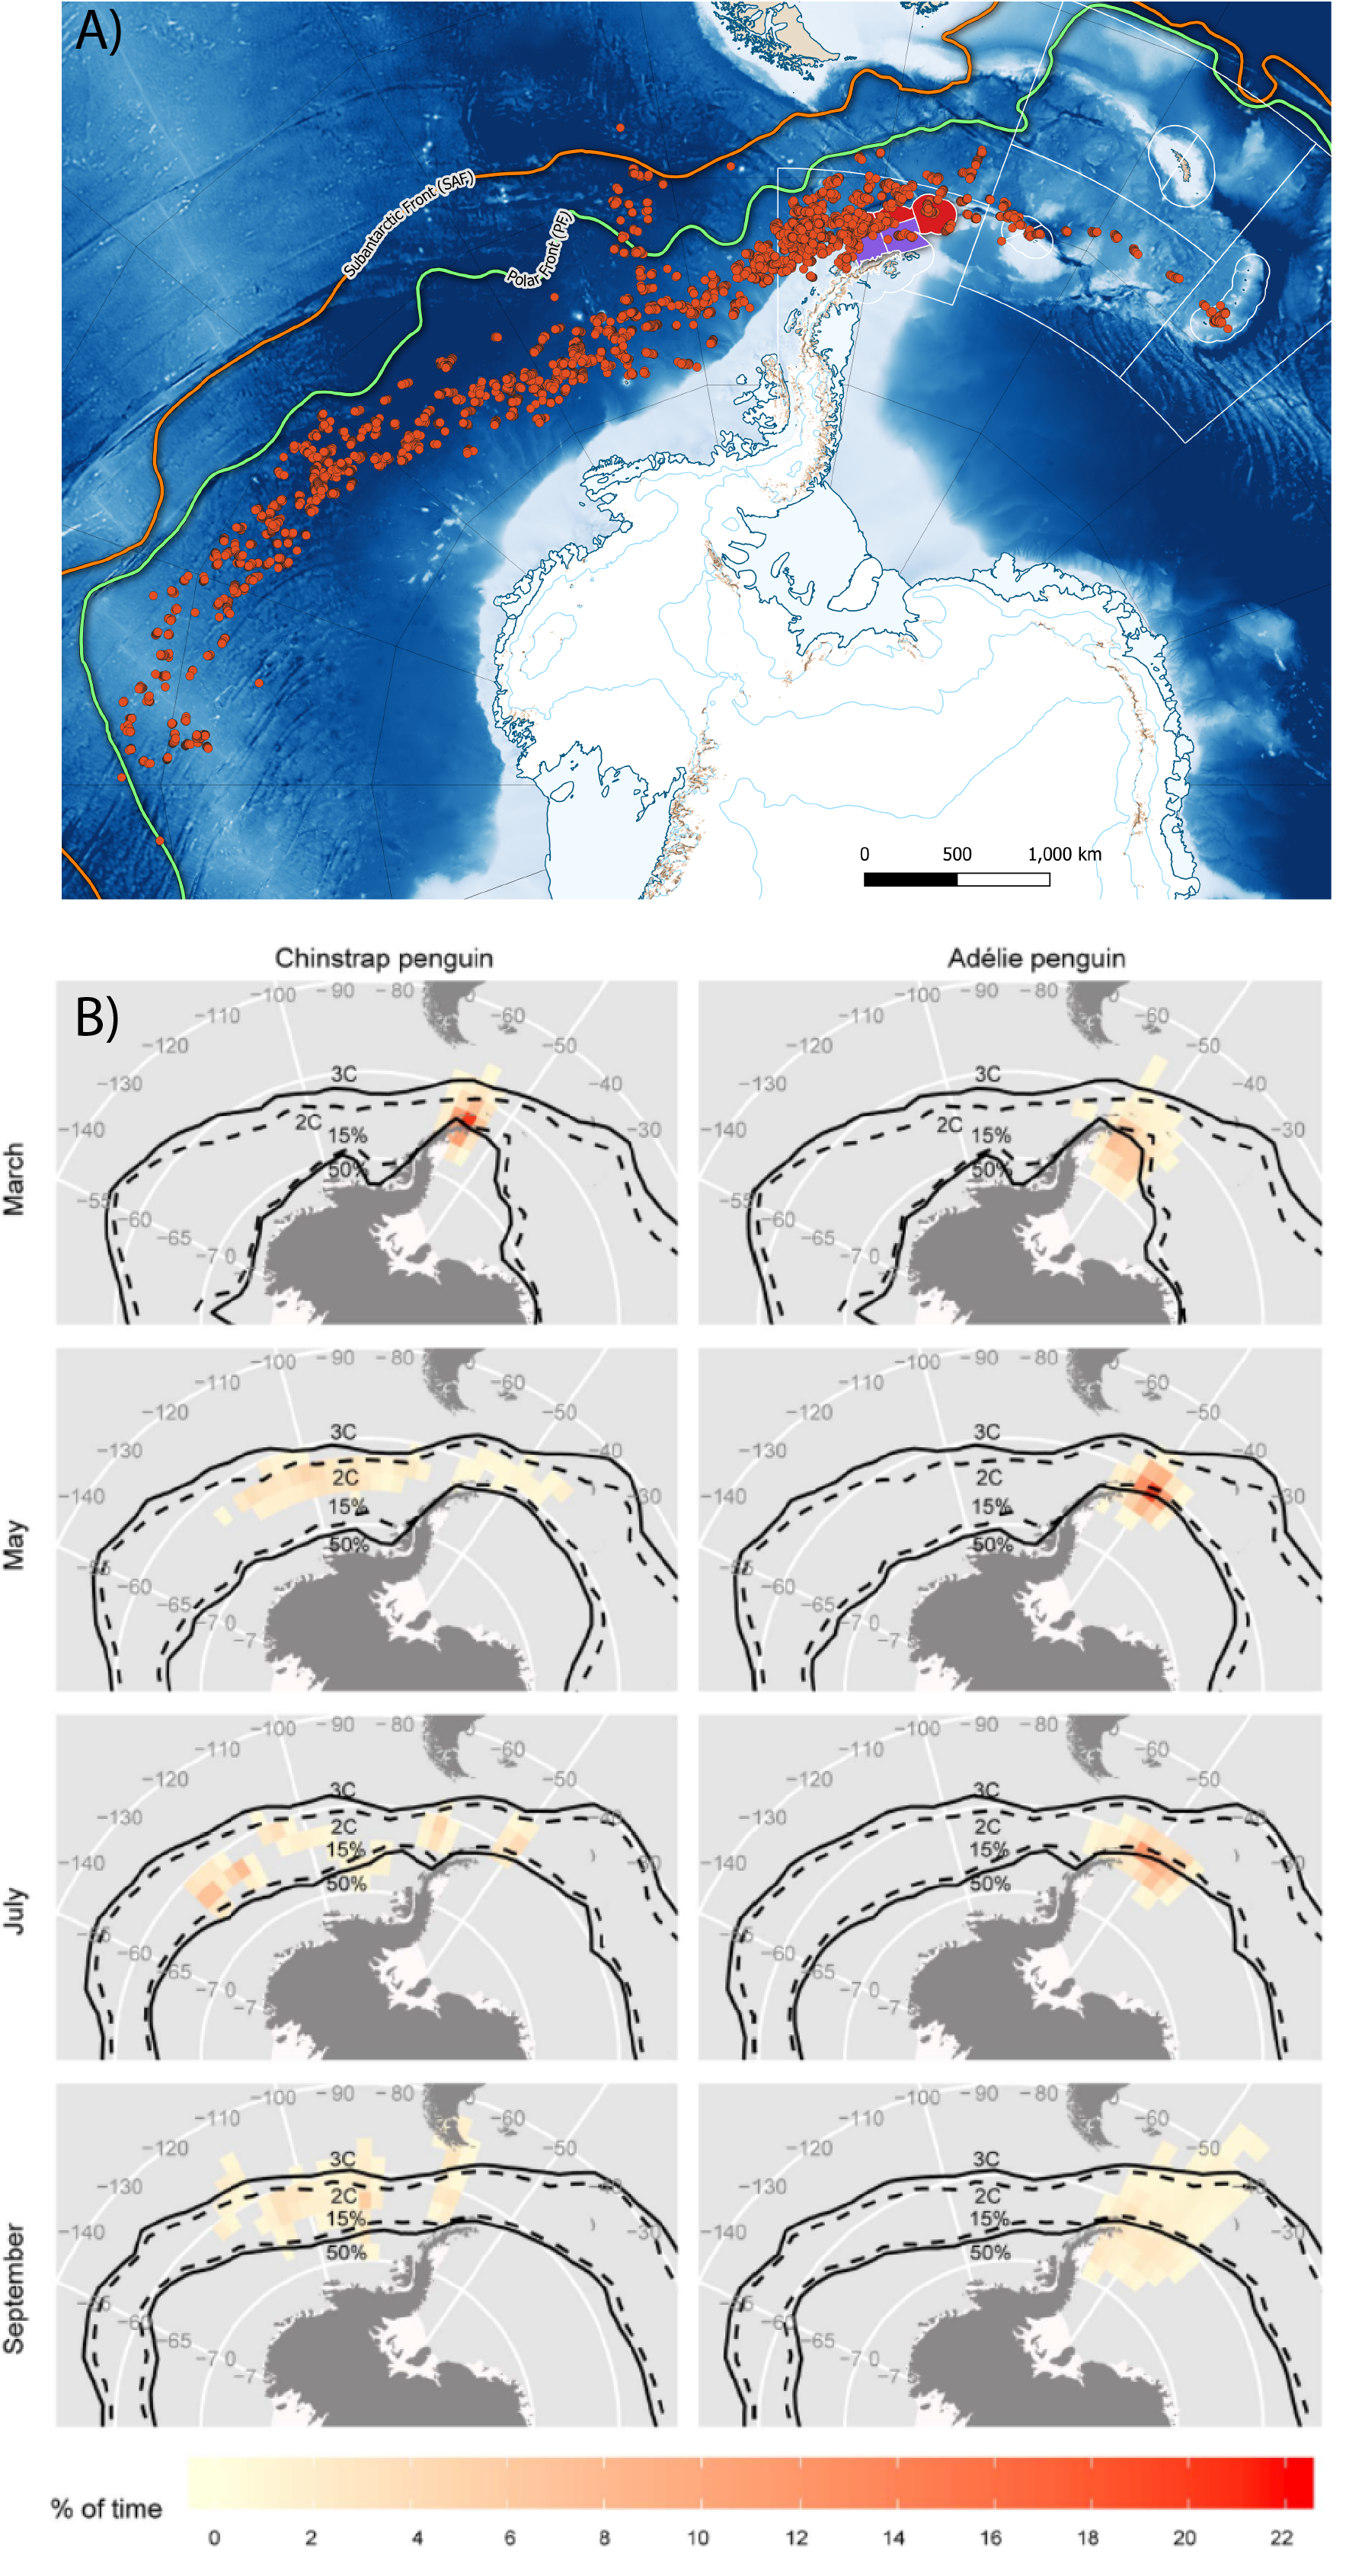
\includegraphics[width=0.75\linewidth]{./Watters EMM figures/Overwinter pengo distributions} \caption{A) Distribution of overwinter movement for chinstrap penguins, relative to the gSSMU's to which they were attributed, created from telemetry data available in Hinke et al. 2019.  B) Adélie and chinstrap penguin movement recorded by light geolocators, highlighting the large longitudinal range both species disperse through at the end of breeding (taken from Hinke et al. 2015).  In the original model formulation by Watters et al. 2020, the winter performance indices for both species are matched to macroscale levels of ONI variability but gSSMU-scale estimates of LKB and LHR.}\label{fig:Overwinter penguin  plots}
\end{figure}

\begin{figure}
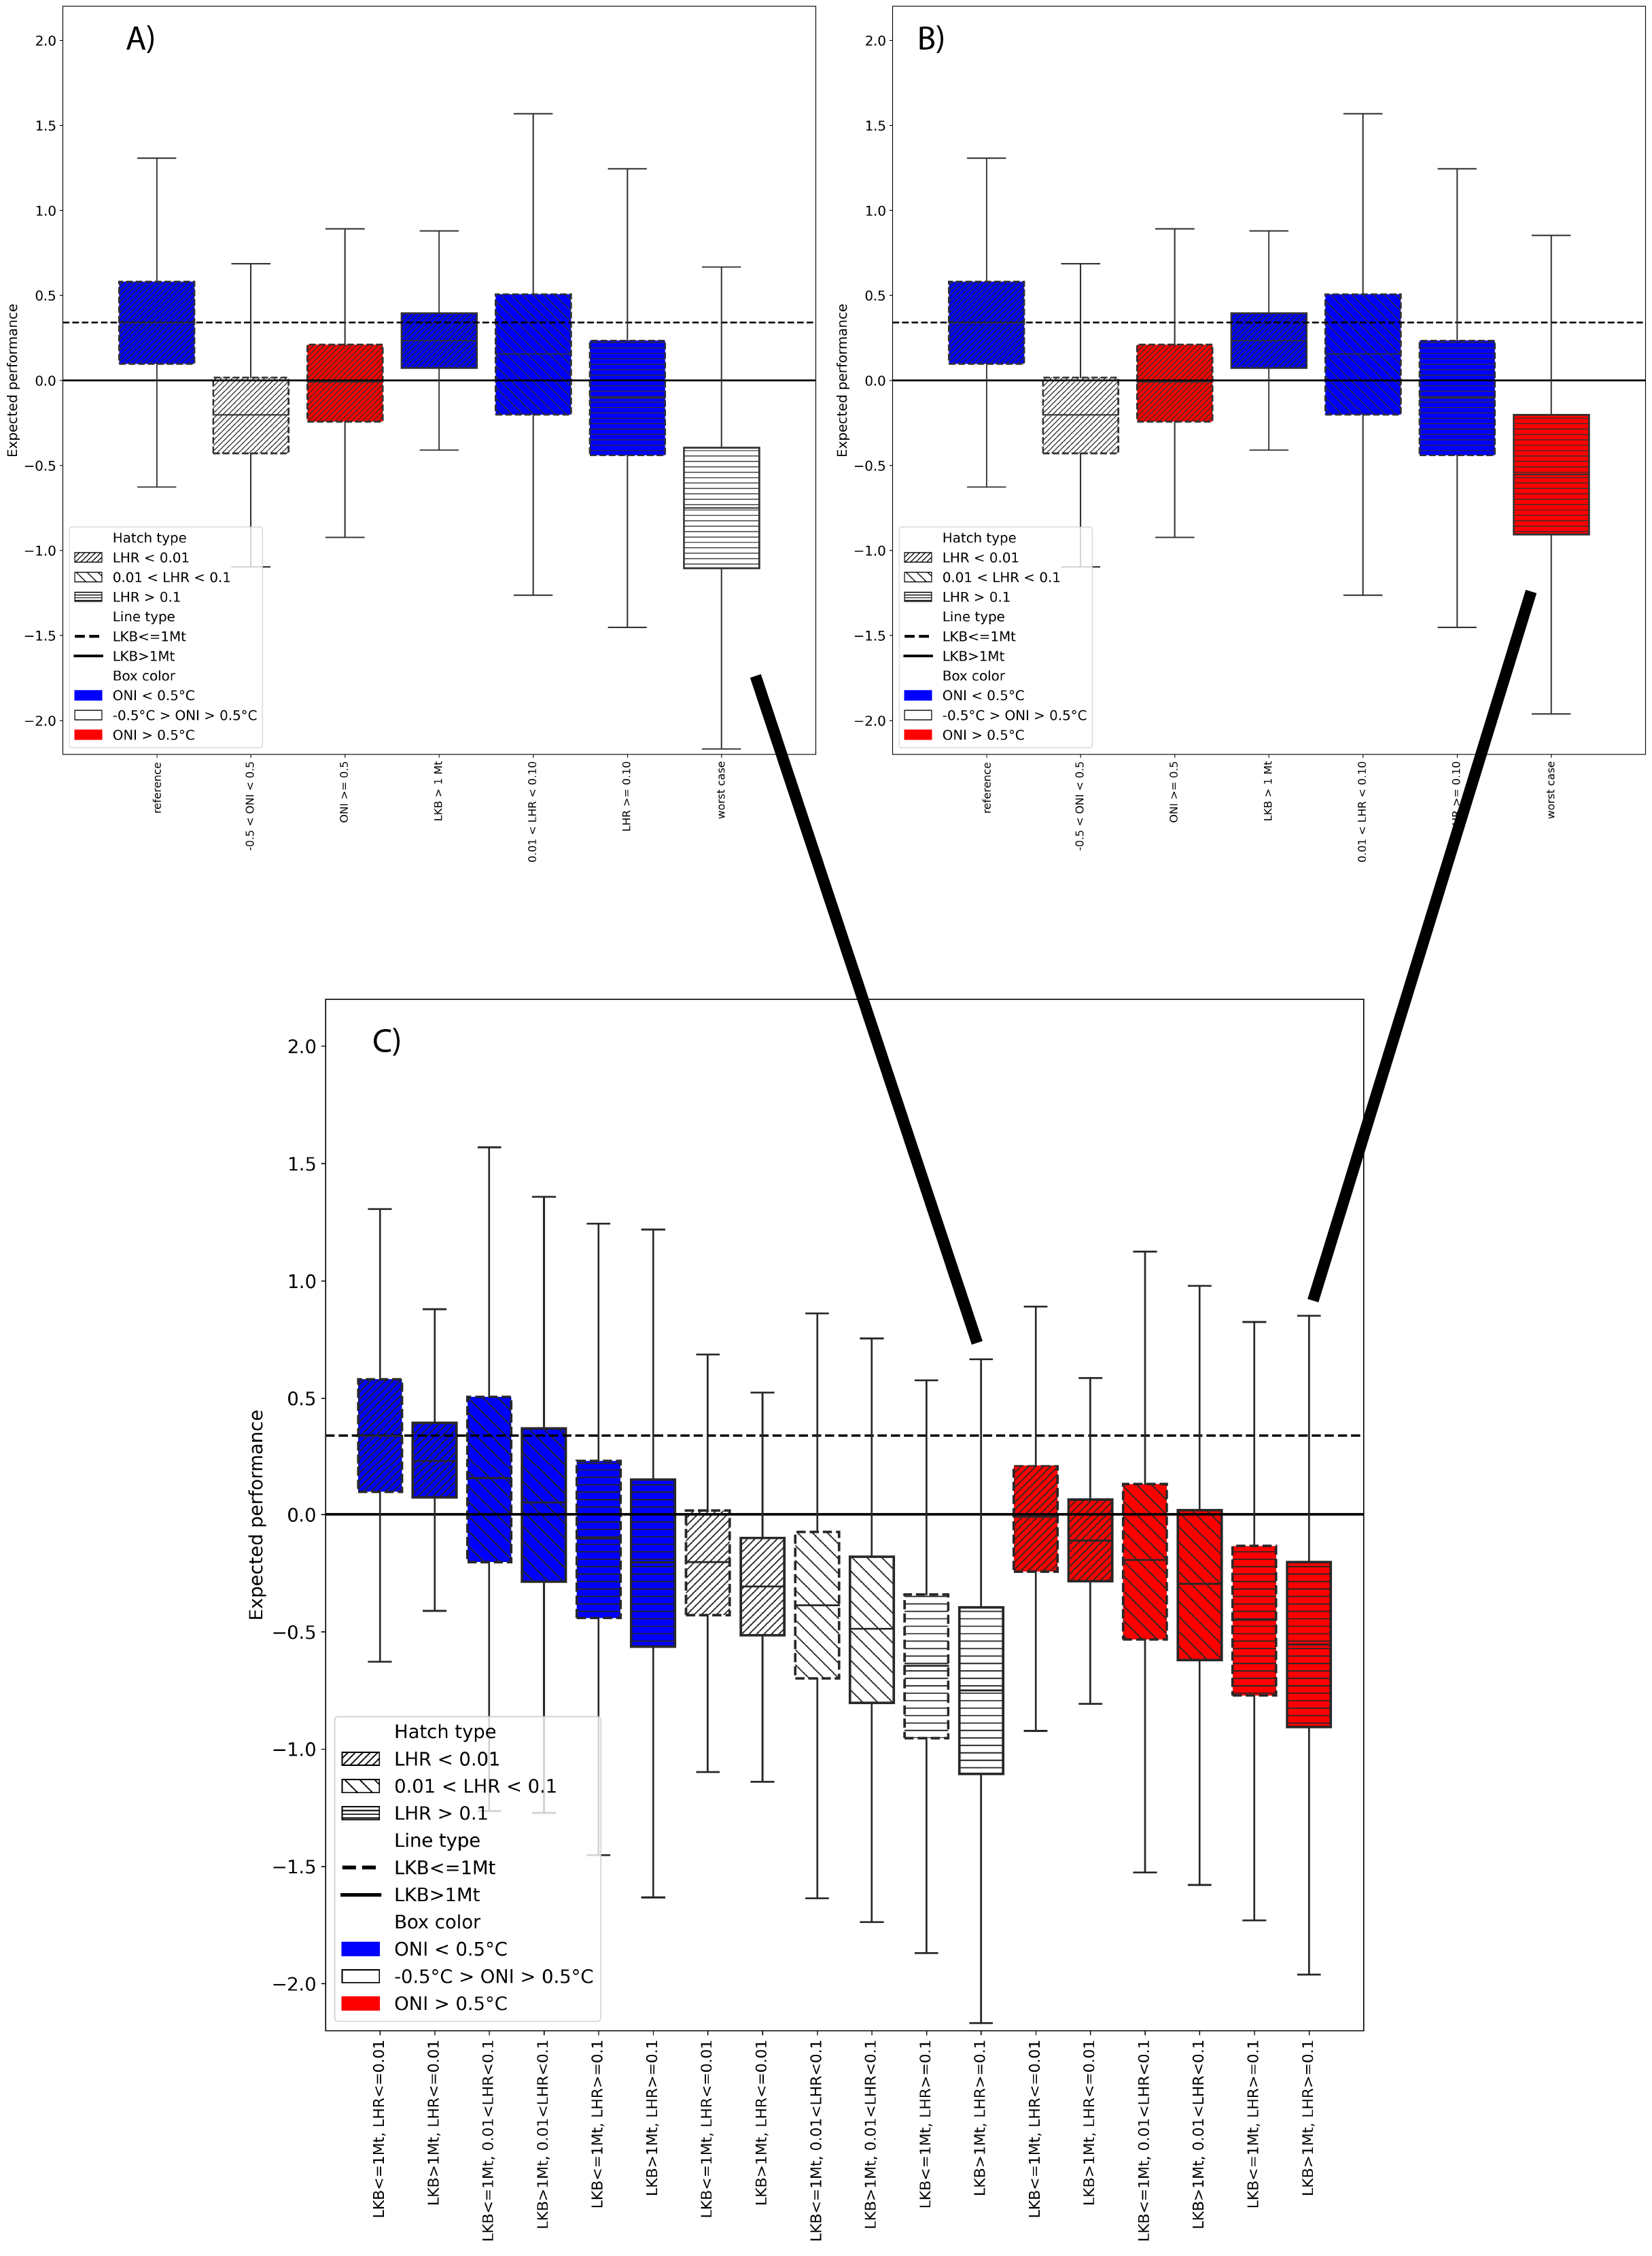
\includegraphics[width=0.75\linewidth]{./Watters EMM figures/Watters original and mistake} \caption{Original Figure 1 plot from Watters et al. 2020 with A) Neutral ONI and B) B) Warm ONI constituting the Worst Case selected.  C) Displays the original case-by-case plots recreated from the paper, with Case 12 representing the intention while data from Case 18 was selected for rendering the boxplot.  Note that the expected performance under neutral ONI Worst Case is poorer than under the warm ONI that was presented in the original paper.  Henceforth, to facilitate comparison, we refer to the ONI Neutral plot however we consider this unrealistic if the intention is to portray a Worst Case of a continuing warming climate.}\label{fig:Watters original and mistake}
\end{figure}

\begin{figure}

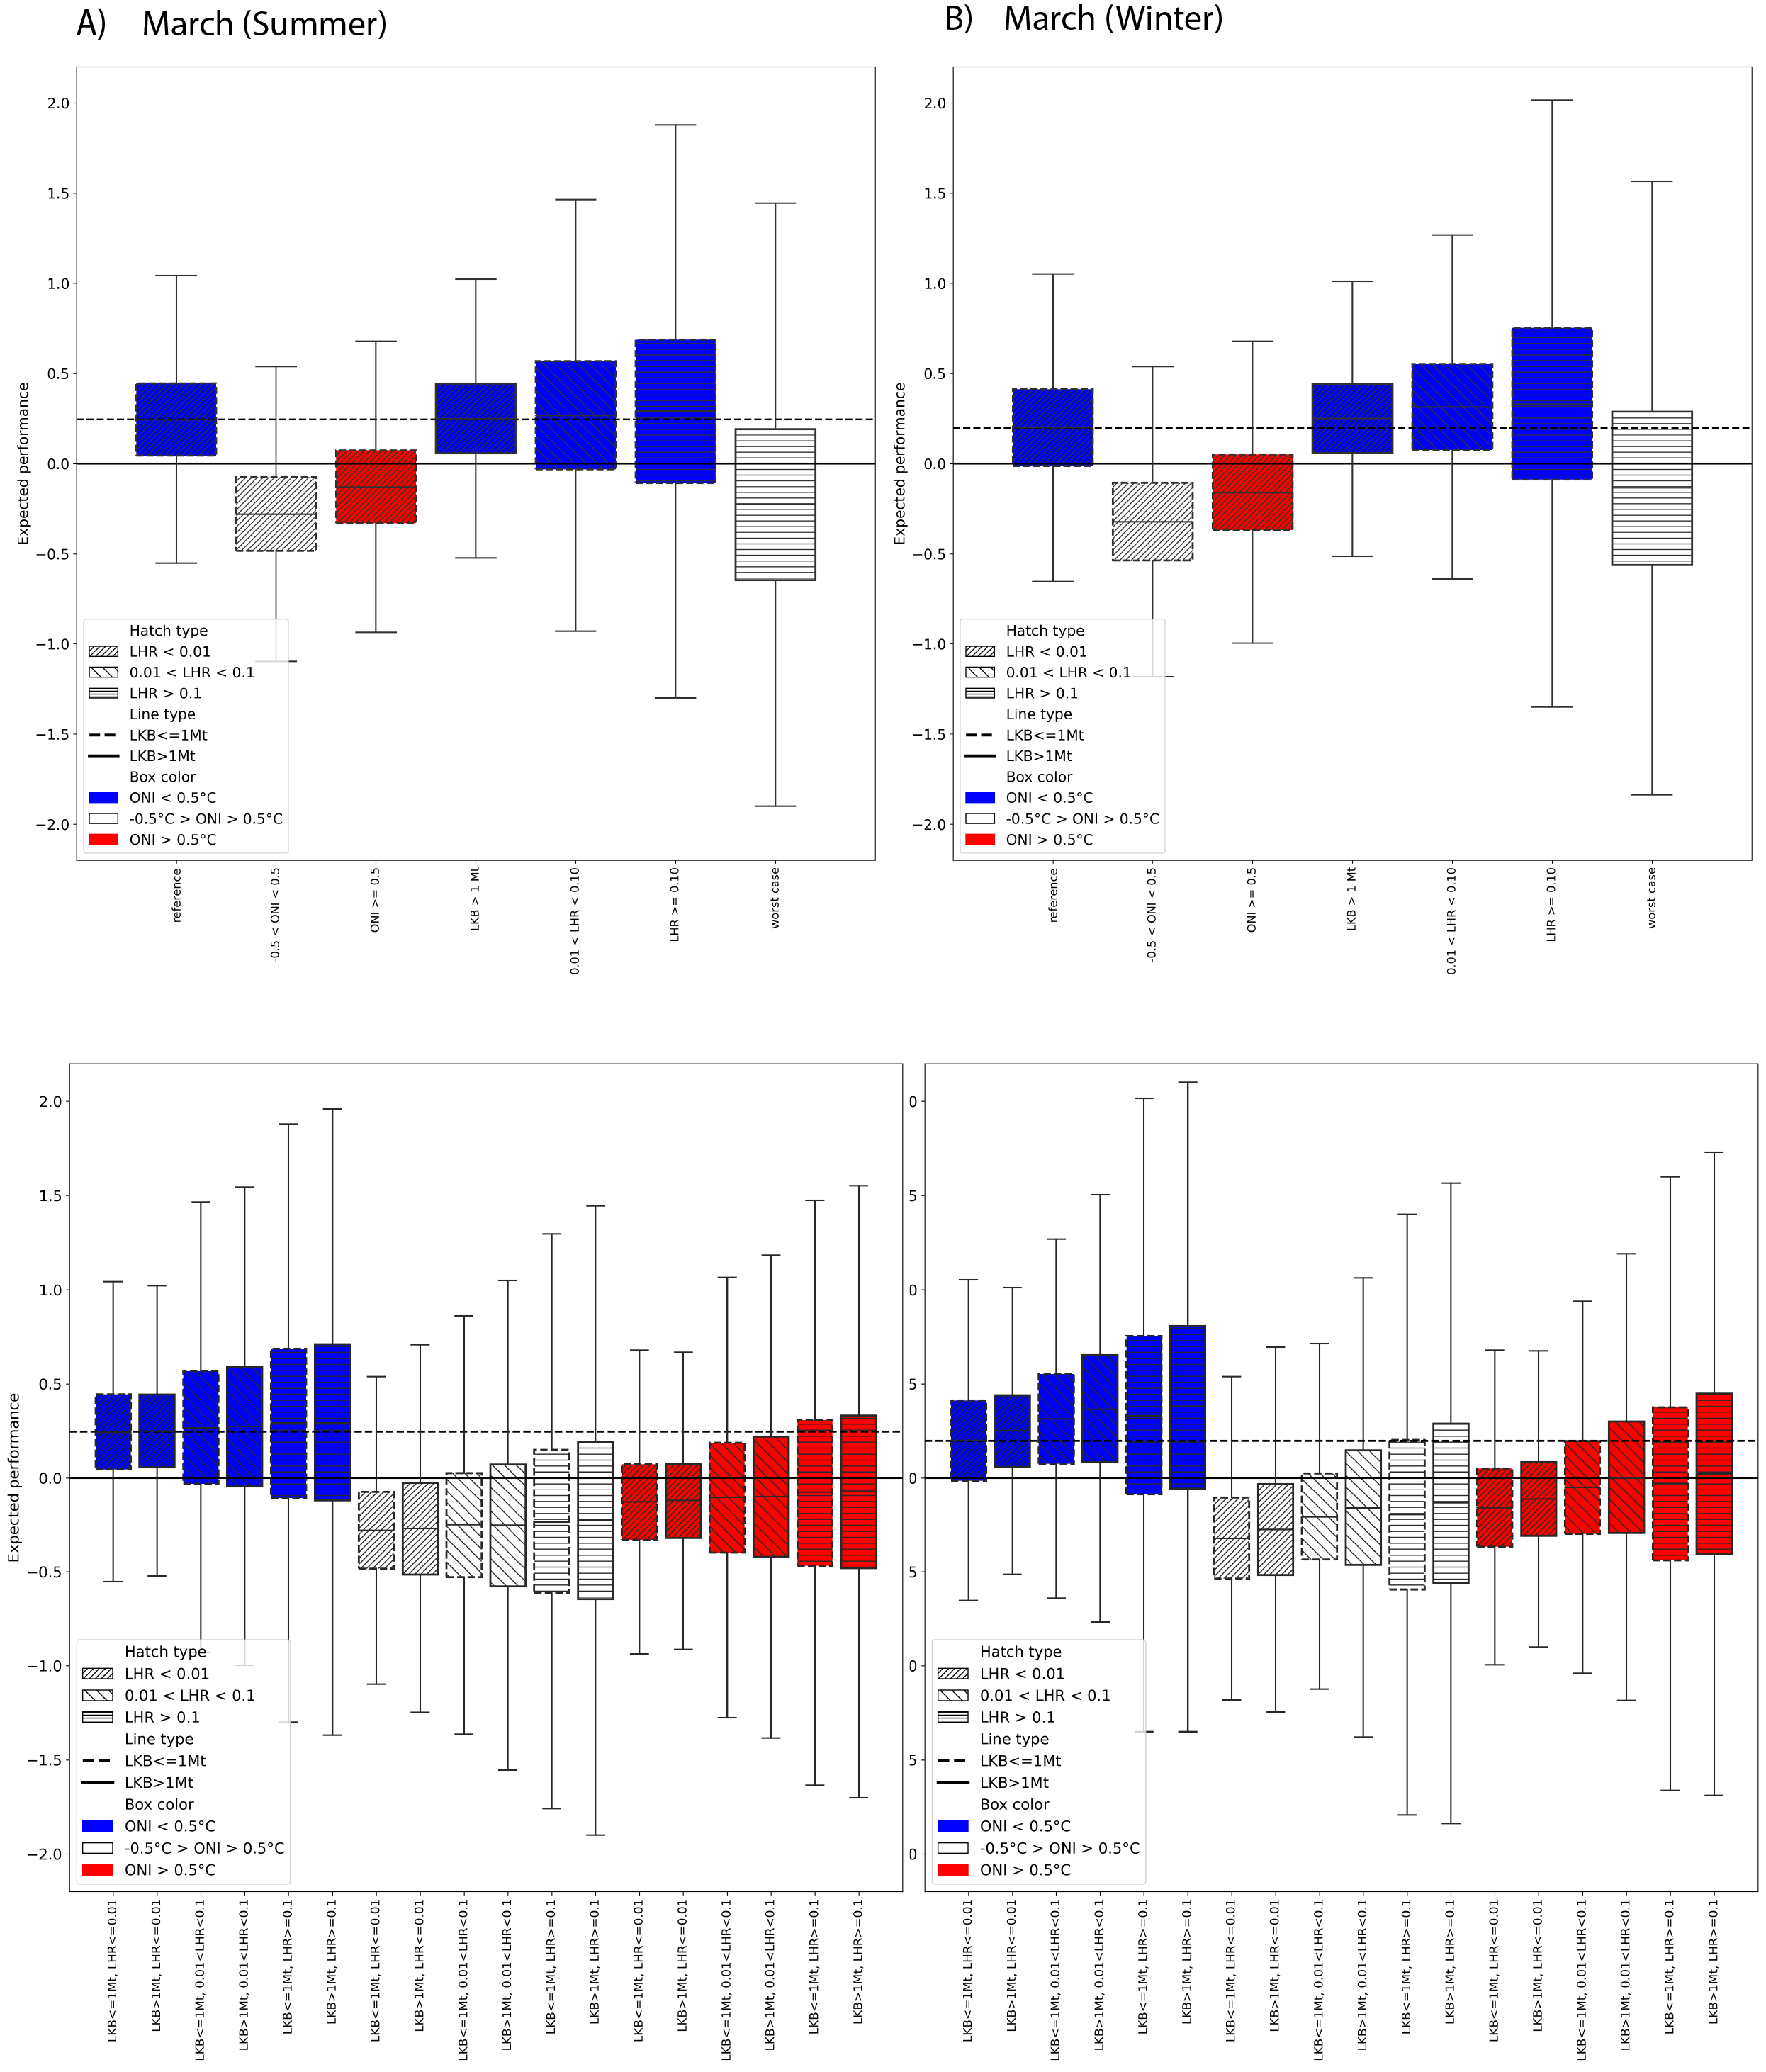
\includegraphics[width=1\linewidth]{./Watters EMM figures/All spp summer then winter 37} \hfill{}

\caption{Model output for the alternatve Watters et al. 2020 scenario outlined above (all species initially present, Adélie and chinstrap penguins migrate out of the area after breeding, LKB and LHR rescaled to SSMU and March included in summer or winter).   Selected cases as per Watters et al. 2020 for March in A) Summer and B) Winter are provided, with the corresponding case-by-case boxplots presented beneath.  Boxplots are colour-coded by ONI state (red=warm, white=neutral, blue=cold).  In all cases, the marginal effect of ONI dominated the expected performance of penguins against their long-term mean, irrespective of LKB or LHR.}\label{fig:Scenario plot 1}
\end{figure}

\begin{landscape}

\begin{longtable}[t]{lccccc}
\caption{\label{tab:Table 1 Scenario Original}Original table in Watters et al. 2020.  In this and all subsequent tables below, the posterior and posterior predictive probabilities that the expected performance of penguins given the effects in the left hand column are less than the expected performance given the drivers in the column headings are provided. Worst Case is represented by neutral ONI; LHR  $\geqslant$ 0.1; and LKB $\geqslant$ 1Mt.  The Best Case is represented by La Niña conditions, low LKB and low LHR.}\\
\toprule
Effects & Best Case & -0.5 \$\textasciicircum{}\textbackslash{}circ\$ C < ONI < +0.5 \$\textasciicircum{}\textbackslash{}circ\$ C & ONI \$\textbackslash{}geqslant+0.5\$ & Long-term \$\textbackslash{}mu\$ & Long-term predicted \$\textbackslash{}mu\$\\
\midrule
Best case & NA & NA & NA & 0.04 & 0.36\\
ONI Neutral & 1.00 & NA & NA & 0.89 & 0.59\\
ONI warm & 0.99 & NA & NA & 0.52 & 0.51\\
LKB High & 0.71 & 0.02 & 0.12 & 0.01 & 0.41\\
LHR medium & 0.75 & 0.16 & 0.31 & 0.32 & 0.44\\
\addlinespace
LHR high & 0.93 & 0.39 & 0.61 & 0.64 & 0.54\\
Worst case & 0.99 & NA & NA & 0.99 & 0.78\\
\bottomrule
\end{longtable}

\begin{longtable}[t]{lccccc}
\caption{\label{tab:Table 1 Scenario 37a}Posterior and posterior predictive probabilities extracted from the model output for alternatve Watters et al. 2020 scenario outlined above with March attributed to winter (Adélie and chinstrap penguins migrate out of the area after breeding, LKB and LHR rescaled to SSMU). Under this scenario, performance against the long term mean is worst for neutral and warm ONI conditions.}\\
\toprule
Effects & Best Case & -0.5 \$\textasciicircum{}\textbackslash{}circ\$ C < ONI < +0.5 \$\textasciicircum{}\textbackslash{}circ\$ C & ONI \$\textbackslash{}geqslant+0.5\$ & Long-term \$\textbackslash{}mu\$ & Long-term predicted \$\textbackslash{}mu\$\\
\midrule
Best case & NA & NA & NA & 0.04 & 0.40\\
ONI Neutral & 1.00 & NA & NA & 0.97 & 0.62\\
ONI warm & 0.99 & NA & NA & 0.81 & 0.56\\
LKB High & 0.49 & 0.01 & 0.05 & 0.03 & 0.40\\
LHR medium & 0.46 & 0.04 & 0.09 & 0.14 & 0.39\\
\addlinespace
LHR high & 0.45 & 0.10 & 0.16 & 0.23 & 0.39\\
Worst case & 0.84 & NA & NA & 0.71 & 0.59\\
\bottomrule
\end{longtable}

\end{landscape}
\begin{landscape}

\begin{longtable}[t]{lccccc}
\caption{\label{tab:Table 1 Scenario 37b}Posterior and posterior predictive probabilities extracted from the model output for alternatve Watters et al. 2020 scenario outlined above with March attributed to summer (Adélie and chinstrap penguins migrate out of the area after breeding, LKB and LHR rescaled to SSMU). Under this scenario performance against the long term mean is also worst for neutral and warm ONI conditions.}\\
\toprule
Effects & Best Case & -0.5 \$\textasciicircum{}\textbackslash{}circ\$ C < ONI < +0.5 \$\textasciicircum{}\textbackslash{}circ\$ C & ONI \$\textbackslash{}geqslant+0.5\$ & Long-term \$\textbackslash{}mu\$ & Long-term predicted \$\textbackslash{}mu\$\\
\midrule
Best case & NA & NA & NA & 0.10 & 0.42\\
ONI Neutral & 1.00 & NA & NA & 0.98 & 0.63\\
ONI warm & 0.99 & NA & NA & 0.86 & 0.56\\
LKB High & 0.40 & 0.00 & 0.04 & 0.03 & 0.40\\
LHR medium & 0.27 & 0.01 & 0.02 & 0.04 & 0.37\\
\addlinespace
LHR high & 0.37 & 0.08 & 0.13 & 0.21 & 0.38\\
Worst case & 0.76 & NA & NA & 0.63 & 0.55\\
\bottomrule
\end{longtable}

\end{landscape}
\begin{landscape}

\end{landscape}
\begin{landscape}

\end{landscape}

\newpage
\setcounter{table}{0}  \renewcommand{\thetable}{S\arabic{table}}     -   - \setcounter{figure}{0} \renewcommand{\thefigure}{S\arabic{figure}}
\begin{landscape}

\section{Supplementary material}\label{supplementary-material}

\begin{figure}
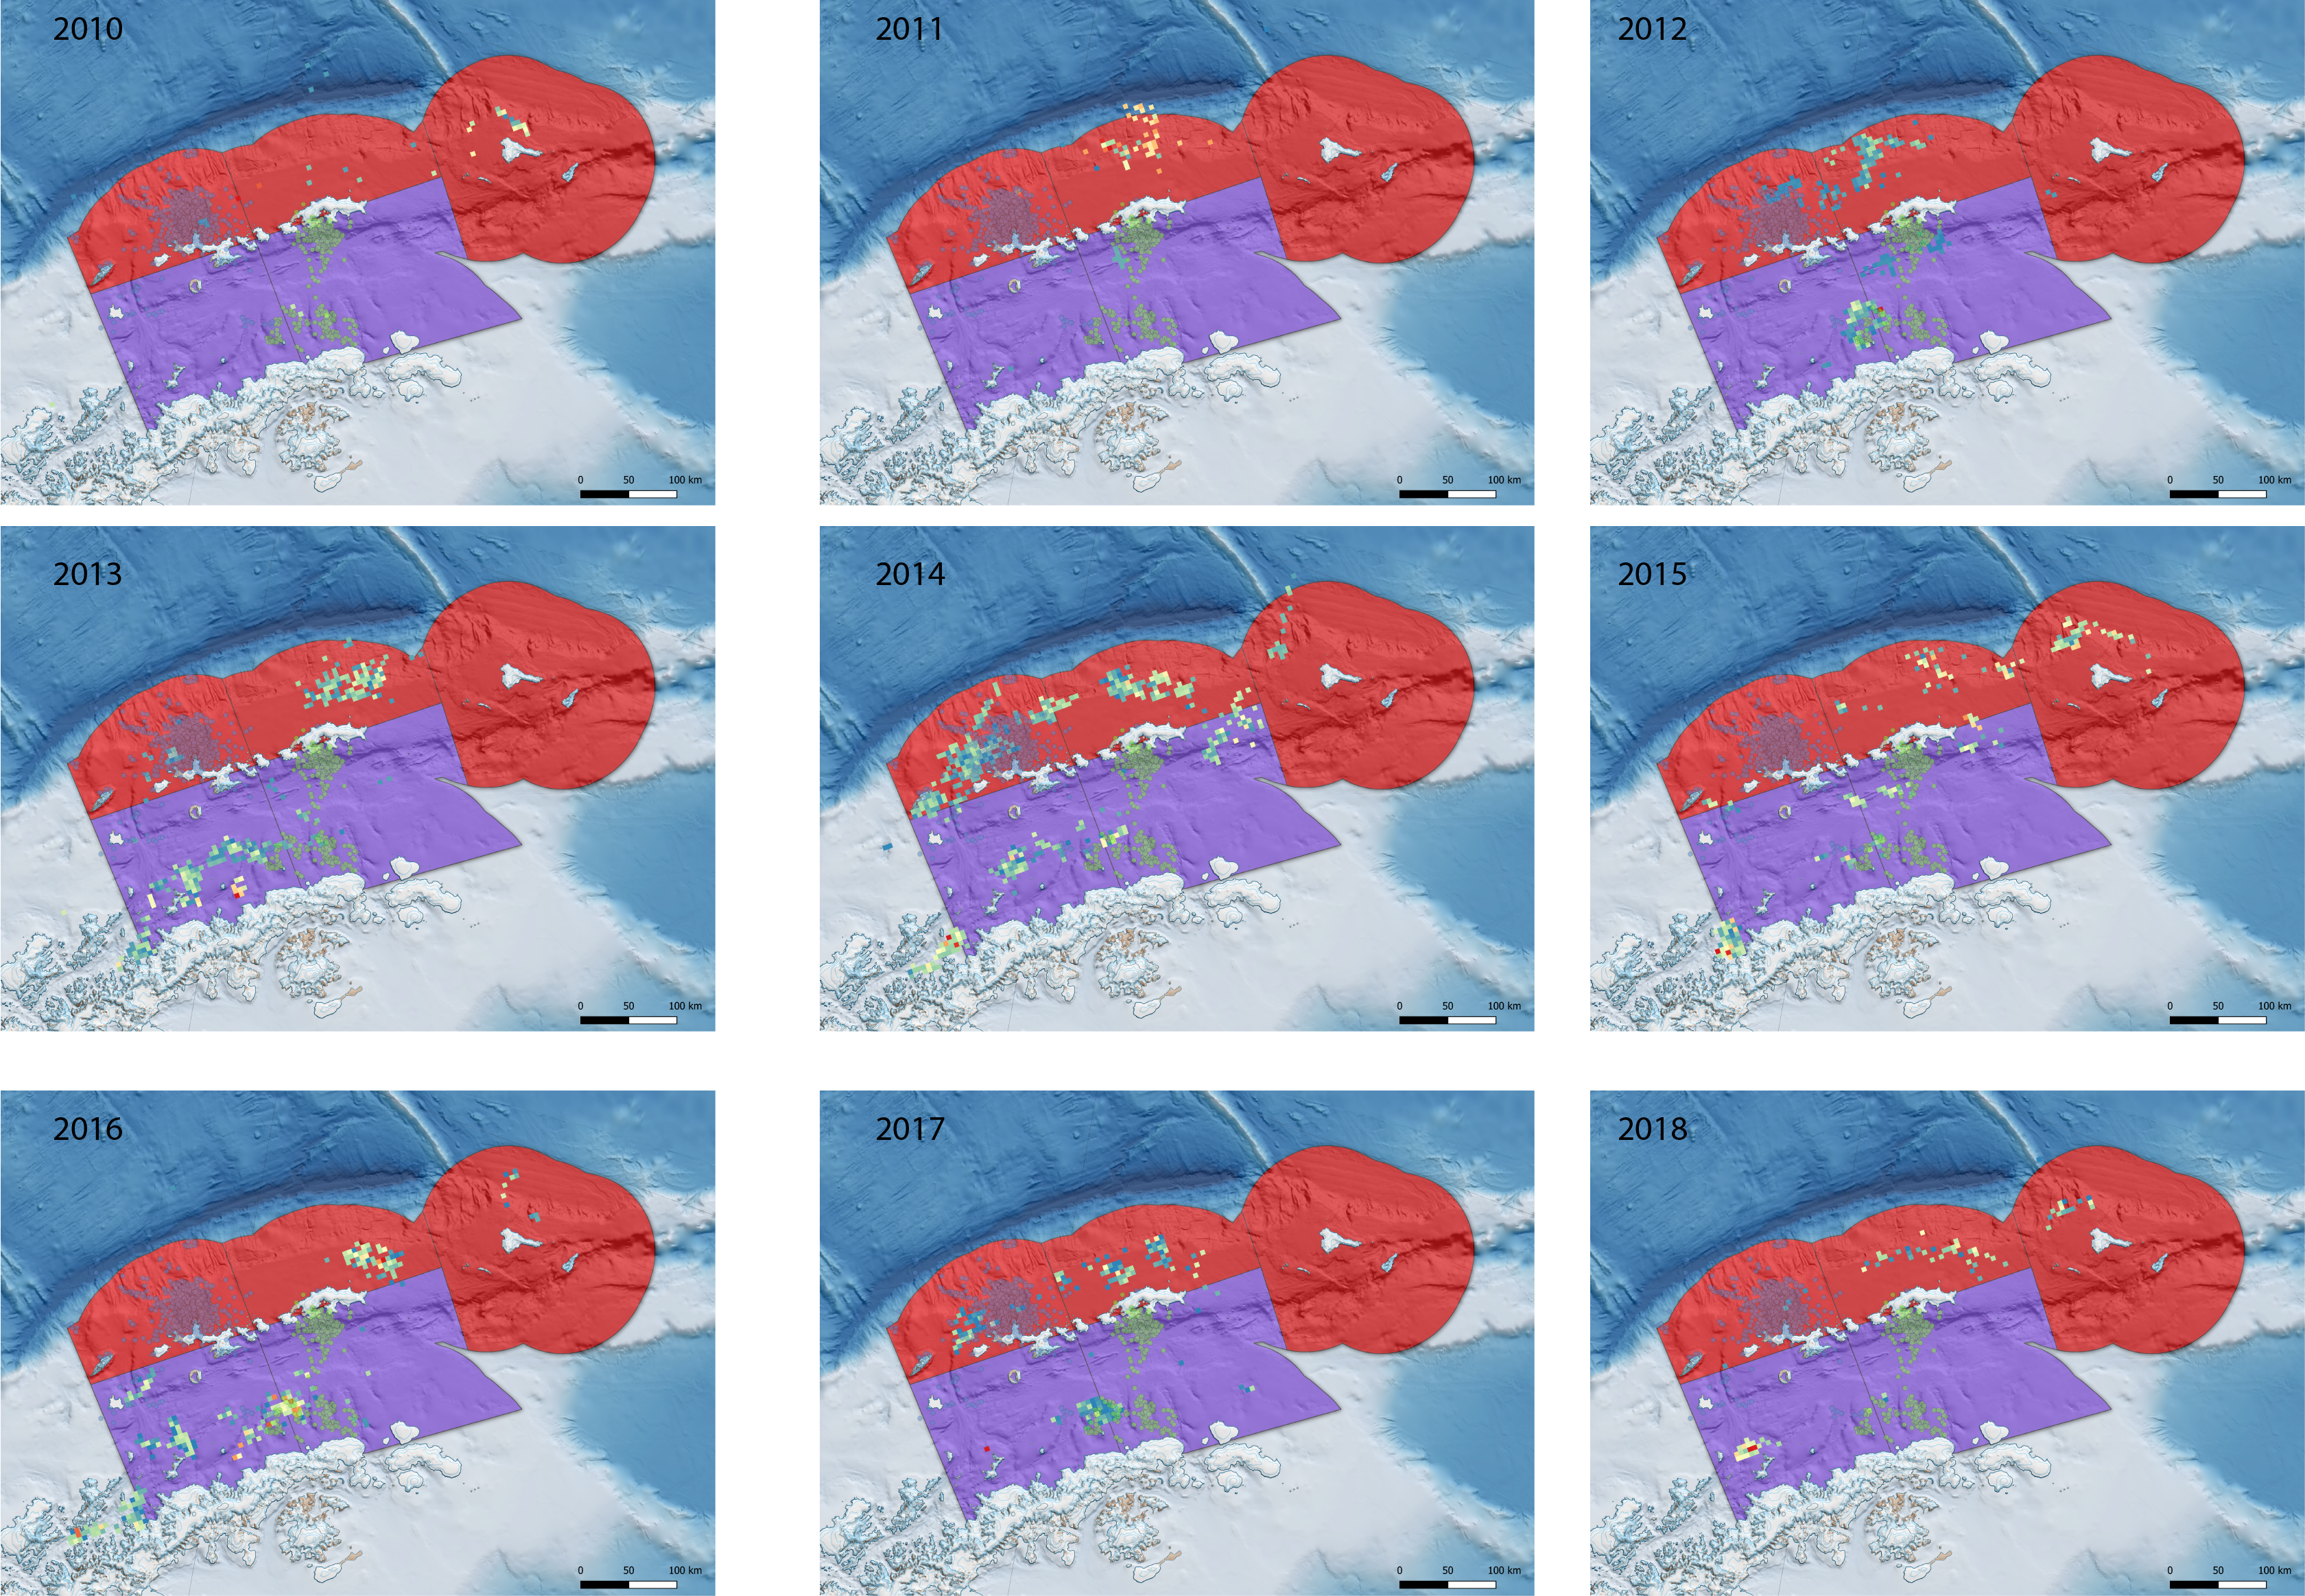
\includegraphics[width=0.8\linewidth]{./Watters EMM figures/summer catch/Year by year catch} \caption{C1 Catch and Effort data for 2010 - 2018, for all catches during the period of the austral summer relating to Adélie and chinstrap penguins in Subarea 48.1 (i.e. up to $10^{th}$ March).  The telemetry data presented in Hinke et al. 2017 for chinstrap penguins at both Cape Shireff and Copacabana and the gSSMU used in the Watters et al. 2020 paper are superimposed to highlight the extreme variability in actual catch, relative to the scale of LHR used to reflect interactions with penguins.  Our reanalysis re-scaled LHR to the SSMU level, though we contend that for the purposes of matching predator data at appropriate spatial scales even this is too coarse a resolution.}\label{fig:Supplementary Figure 1}
\end{figure}

\end{landscape}

\begin{figure}

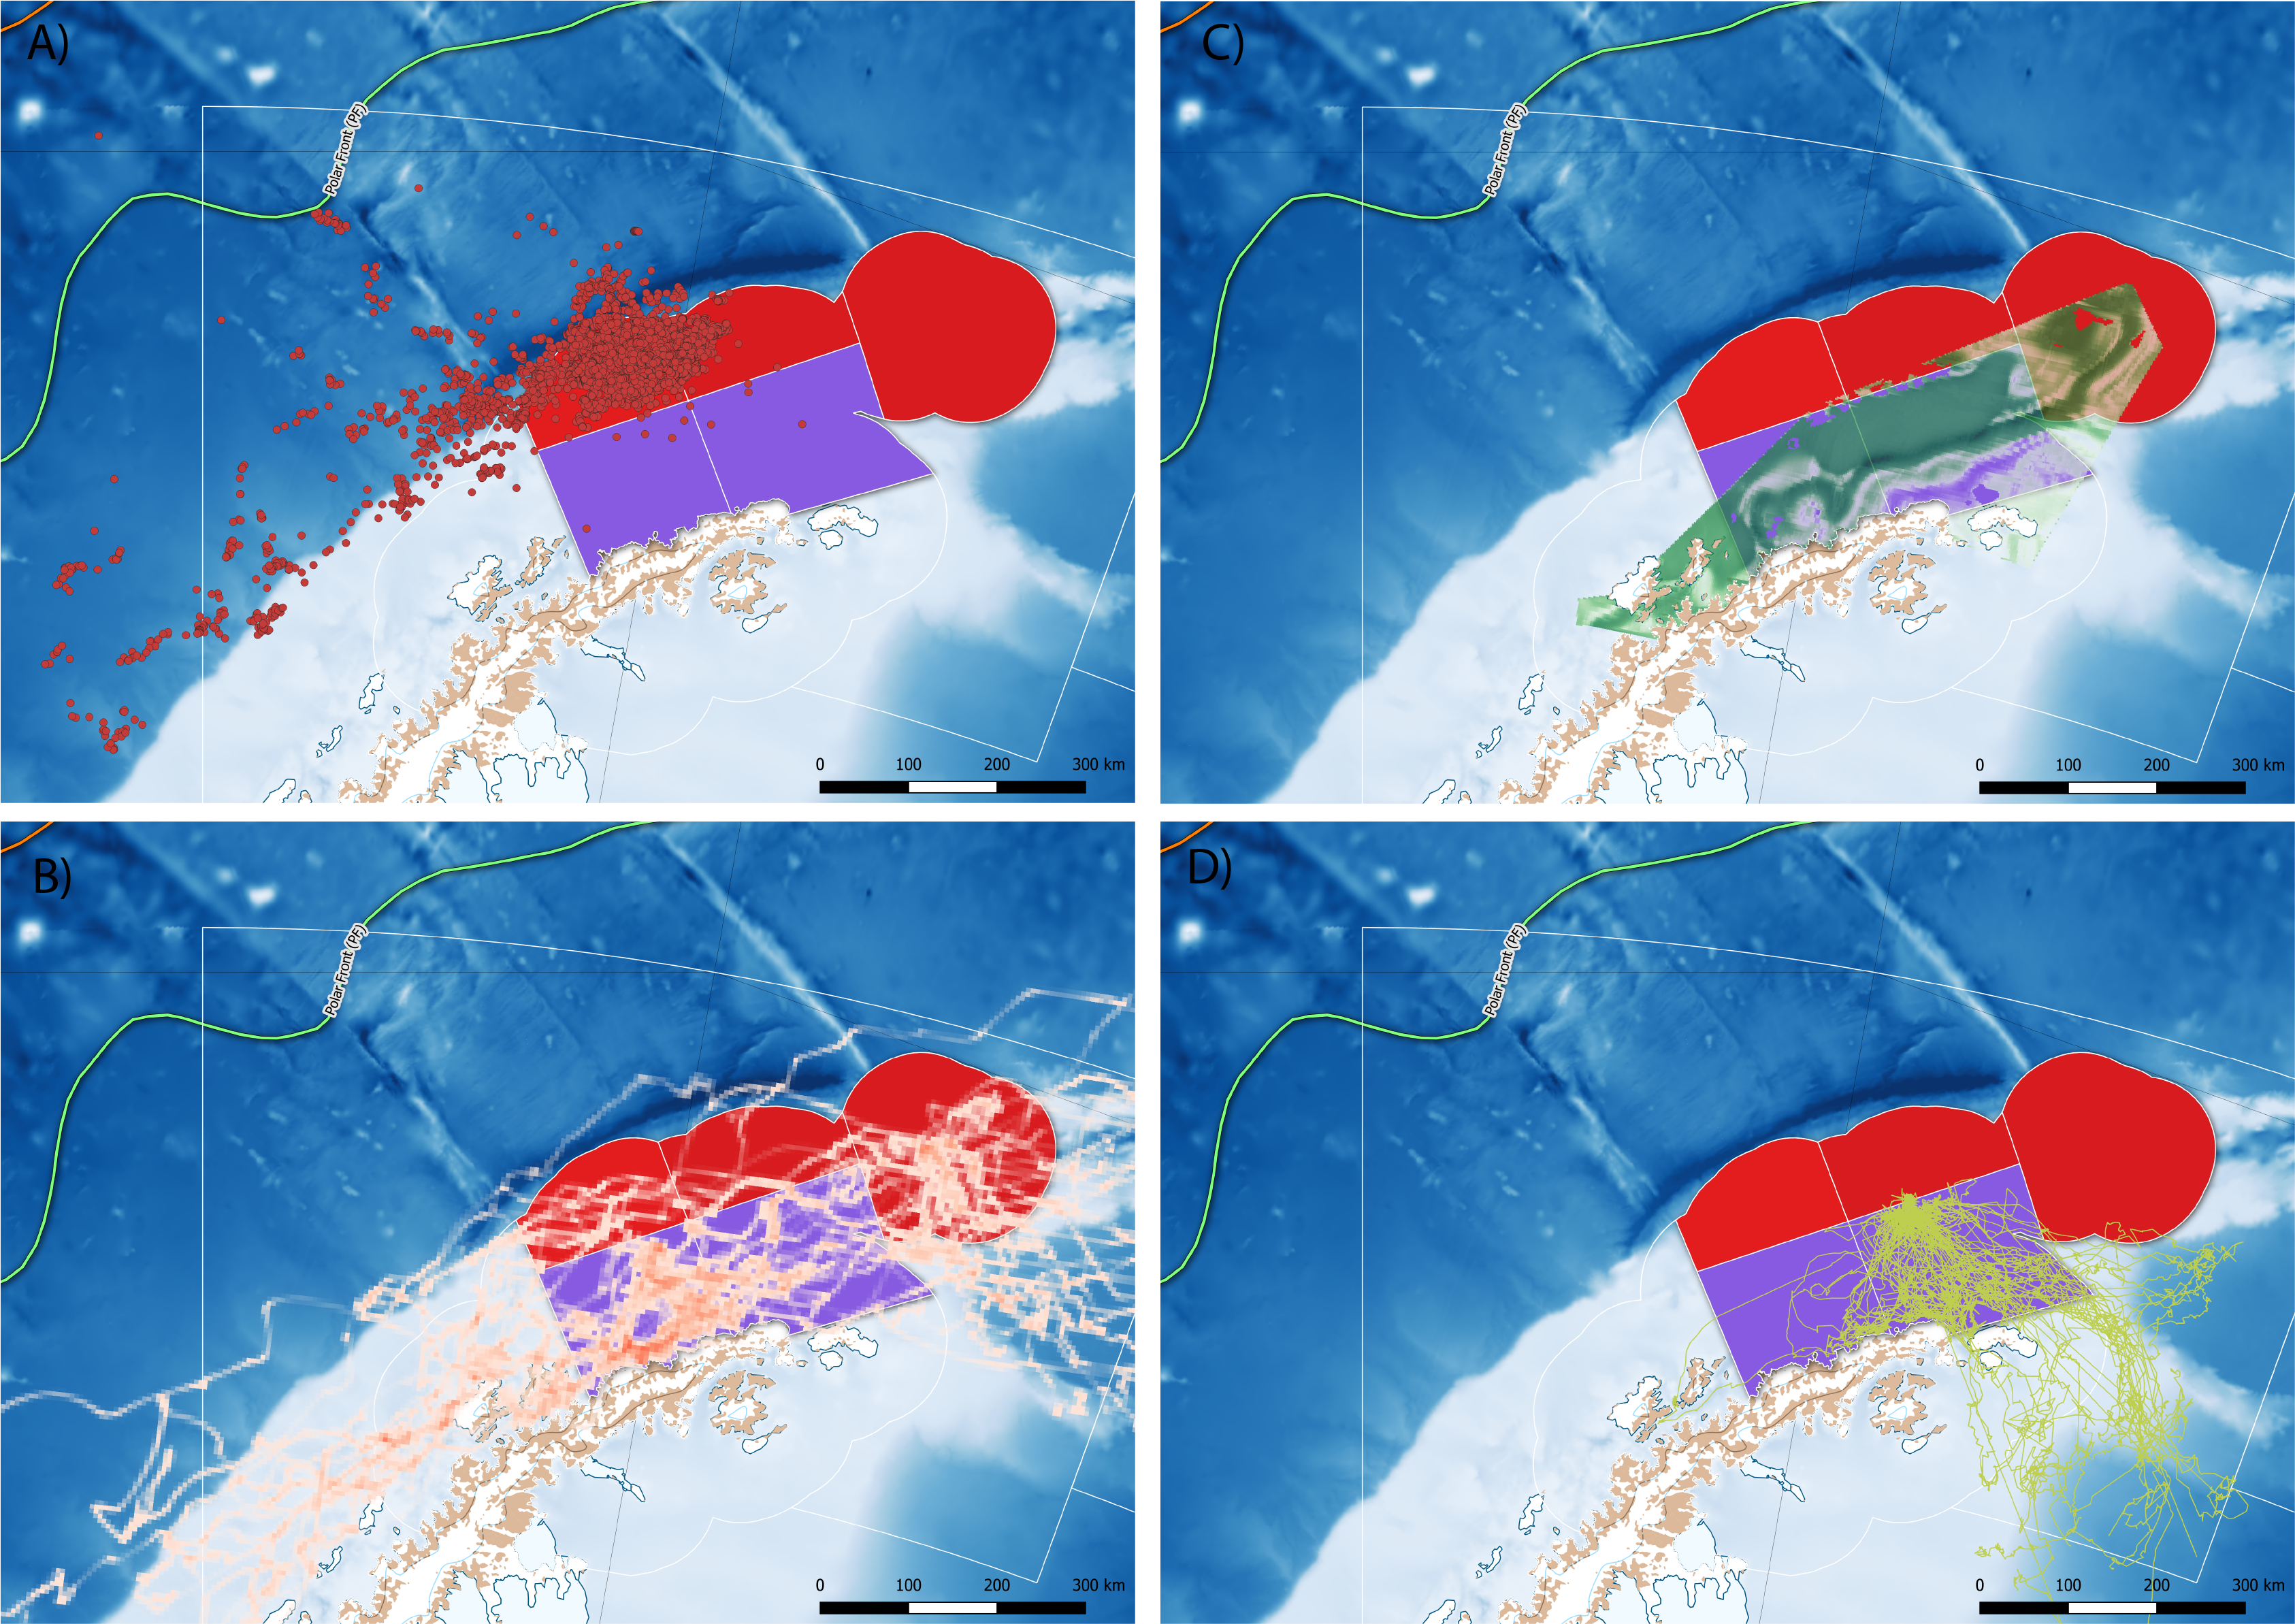
\includegraphics[width=1\linewidth]{./Watters EMM figures/Other spp distribution} \hfill{}

\caption{The summer distribution of foraging effort by A) adult female Antarctic fur seals (adapted from telemetry data available in Hinke et al. 2017), B) migratory adult male Antarctic fur seals (adapted from Lowther et al. 2020) C) humpback whales throughout December (adapted from Johannessen et al., this meeting) and D) nonbreeding adult Adélie penguins during the breeding season (adapted from data in Oosthuizen et al., this meeting). Potential effects of competitive overlap between pygoscelid penguins and other krill dependent predators, particularly those who have increased their abundance dramatically over the preceding 40 years, are excluded from both approaches, creating an unrealistic set of boundary conditions for interpreting the variance in penguin vital rates.}\label{fig:Supplementary Figure 2 other species plots}
\end{figure}

\newpage

\renewcommand\refname{Citations}
\bibliography{mylib.bib}


\end{document}
